\section{Definition}

\subsection{Project Overview}

This project addresses a problem from the education domain. Its goal is the creation of a framework that can be used by the scientific personnel of a university to evaluate the quality, i.e., the ability to convey scientific topics, of the exercises used throughout the university courses. Please refer to the capstone proposal document to find detailed information about the domain background, the related work and the data set that will be used throughout this project.

\subsection{Problem Statement}\label{la_problem_statement}

The overall vision of this project is depicted in Fig.~3 of the capstone proposal document:

\begin{enumerate}
	\item The tutor provides abstract, subjective descriptions of the problem that is treated in the evaluated exercise and of the students that this exercise is intended for.
	\item In addition to this, the tutor describes the current structure of the exercise that will be used to teach the students to handle the problem at hand.
	\item The trained prediction model (the “Learning effectiveness prediction” block in Fig.~3) takes these inputs and provides a prediction about the effectiveness of the exercise which classifies the structure of the exercise as effective or not. If the exercise is classified as ineffective, the tutor adjusts its structure and performs the next evaluation iteration.
\end{enumerate}

As detailed in the capstone proposal, the problem that is addressed in this project can be divided into three subproblems. 

Training the effectiveness prediction is obviously an important step during the framework creation. However, the data set that is used throughout this project describes the learning process of students that are using an on-line framework to learn algebra related problems. The situation in which the data set was gathered differs from the situation addressed in this project in two important aspects: \textbf{a)} the problems that the students were solving come from a different domain and  \textbf{b)} the data set contains information that will not be accessible for the tutors of a university class, like, e.g., the exact time that was needed for solving the problem steps. Consequently, the data set can not be used for the training of the prediction model without a preprocessing step. During this preprocessing, the detailed data set entries describing the students and the problems have to be mapped onto subjective categories that can be intuitively used by the tutors. A schematic of the three subproblems is given in Fig.~\ref{fig_sub_problems}.

  \begin{figure}
  	\centering
  	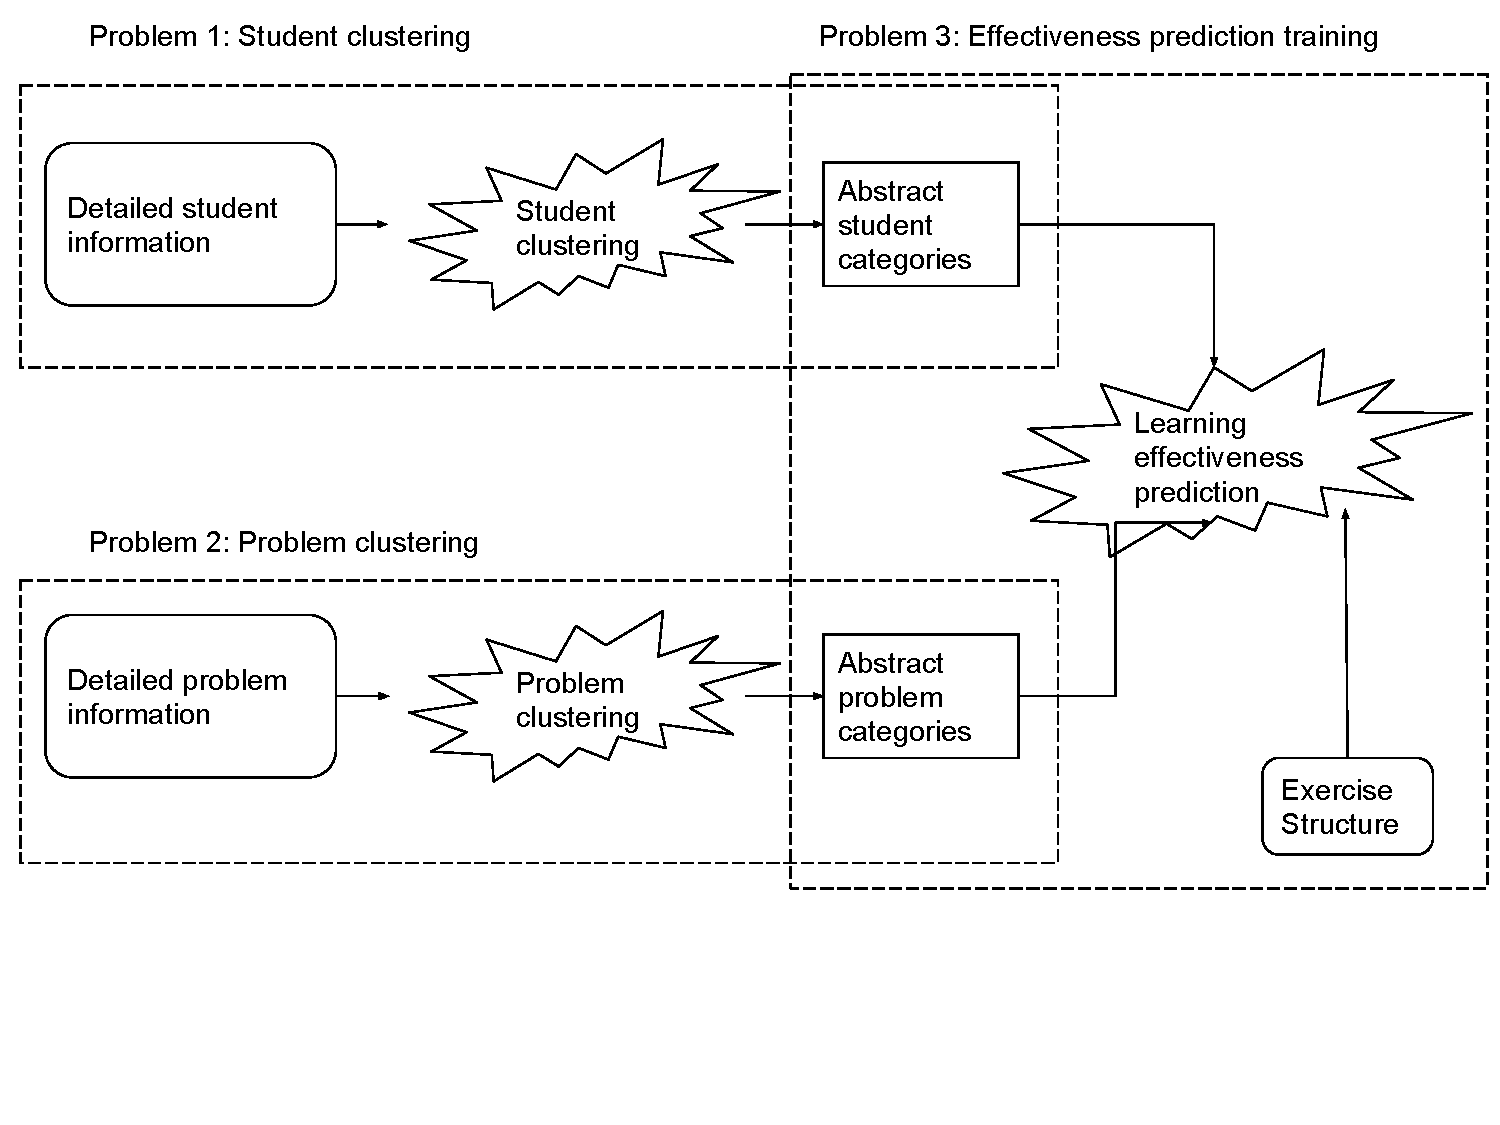
\includegraphics[width=\textwidth]{./img/subProblems.pdf}
  	\caption{The overall problem can be divided into three subproblems \label{fig_sub_problems}}
  \end{figure}
  
Following the recommendation of the reviewer of my capstone proposal, I would like to concentrate on one of the subproblems during the capstone project that I am doing in the scope of the Nanodegree and complete the other problems as a hobby project. The problem I would like to concentrate on is the clustering of the students on the abstract student categories (Problem 1 in Fig.~\ref{fig_sub_problems}).

\paragraph{Problem Description:}

The goal of the student clustering is a mapping, where the attributes from the KDD cup data set (consisting of measurements such as the time for the problem solutions) can be mapped onto more abstract student categories that a tutor would use to describe the skill level of students. In a way, the goal of the student clustering is the creation of a model that allows to transform the measurable attributes found in the KDD data set into the hidden features describing the skill levels of the students.

\paragraph{Problem Approach/Task Outline:}

To create a model capable of clustering the students onto categories describing the students’ skill level, the following tasks have to be carried out:

\begin{enumerate}
	\item Data analysis / Preprocessing
	\item Feature engineering
	\item Clustering
	\item Evaluation
\end{enumerate}

\begin{description}
	\item[Data Analysis] The first step of the student clustering is an analysis of the data provided in the KDD data set. At the very start, I hereby intend to check the data for completeness to rule out the possibility that certain attributes are only present in a small subset of the data, making them useless for the clustering. In the next step, I will gather information describing the overall set (for example the number of individual students or the number of exercises processed by each student). In the final step of the data analysis, I then will check each feature in the KDD set and decide \textbf{a)} whether it is, in my opinion, likely to be relevant to describe the student’s skill level and \textbf{b)} whether this feature is accessible for a tutor trying to assess the skill level of his/her students or not (e.g., the exact time the students need for the exercises that were carried out in the past will not be known to the tutor designing the exercise. On the other hand, the information whether or not the students have seen a  similar problem in the past is something that the tutor is likely to know). This distinction is important, as features that are not accessible for the tutor can not be part of the input provided for subproblem 3 and consequently, have to be transformed onto abstract categories while the accessible features may be directly used by the tutor as input for the learning effectiveness prediction.
	
	\item[Feature Engineering] The goal of the feature engineering step is a transformation of the features of the KDD data set onto the hidden feature describing the skill level of the students. On the one hand, this step will reduce the number of features used as the input for the clustering algorithm, hereby hopefully preventing overfitting. On the other hand, it will create new features describing the students and give me a feeling for the overall qualities that determine the cluster the students are associated with. At this point, I intend to apply PCA and experiment with different numbers of components. The overall goal of the student clustering is to be able to work with categories that are understandable for the tutors. It is consequently very important that the new features created by the feature engineering step can be interpreted with respect to a certain student quality.
	
	\item[Clustering] The goal of the clustering step is to take in the features provided by the feature transformation and use them to cluster the students. The clustering does not necessarily have to be done according to the skill level, but the result has to be interpretable so that the tutors have the possibility to determine the group their students can be assigned to. In this step, I intend to try different clustering algorithms and different sets of features in order and choose which combination delivers the best result. The results hereby will be evaluated based on the confidence with which the students are assigned to different groups and on how well the results can be interpreted and explained by an observable quality of the students.
	
	\item[Evaluation] As the objective of the clustering is to assign students to a skill group, I think a good way to evaluate the results is to examine whether the membership of a student to a skill group correlates with their relative strength within the student group, i.e., their position in a list where the students are ordered based on their relative correctness. 
\end{description}

\subsection{Metrics}

As described in the capstone proposal and in section \ref{la_problem_statement}, I will evaluate the results of the student clustering by comparing them to a list where the students are ordered based on the average correctness that they achieved in the problem steps they carried out. 

I expect that the students that can be found in the same clusters will have a similar position on the correctness list. If the clustering results differ from the correctness list in a significant way, the reason for this difference has to be investigated.

 Although I do expect a certain degree of correlation between the clustering results and the correctness list, I think that a certain degree of difference is also desirable. Otherwise, no clustering would be needed and we could simply use the average exercise correctness to classify the students.